En este capítulo, se presenta el diseño de interfaz de la aplicación desarrollada, y las diferentes opciones que se presentan.
\section{Diseño interfaz y navegación}

En la Figura \ref{fig:Mockup} se presenta un bosquejo de la interfaz del usuario, la cual muestra la simulación principalmente, y además un control flotante. También se muestran los menús desplegables.
\begin{figure}[h]
\centering
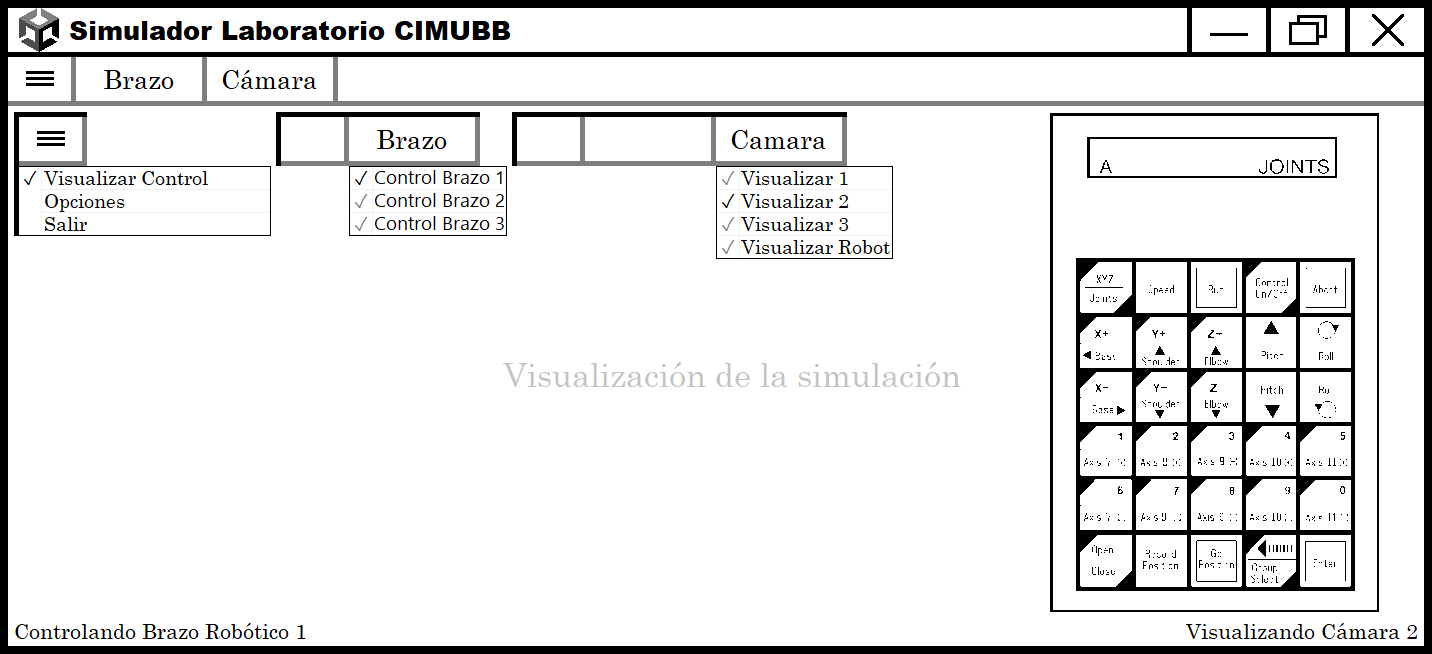
\includegraphics[height=5.82cm]{figures/Mockup.png}
\caption{Diseño interfaz: Módulo Principal}
\label{fig:Mockup}
\end{figure}

Las distintas opciones se detallaran a continuación
\begin{itemize}
\item Menú
    \begin{itemize}
    \item Visualizar Control: Mostrar u ocultar el control flotante
    \item Opciones: Despliega las opciones de programa
    \end{itemize}
\item Brazo: Selecciona el brazo robótico a utilizar
\item Cámara: Selecciona la cámara a visualizar
\end{itemize}